\documentclass[12pt]{article}

\usepackage{sbc-template}
\usepackage{graphicx,url}
\usepackage[utf8]{inputenc}
\usepackage[brazil]{babel}
\usepackage{amsmath}
\usepackage{booktabs}
\usepackage{multirow}

\sloppy

\title{Paralelização da Avaliação de Aptidão em Algoritmos Genéticos
  com OpenMP: Análise de Speedup, Eficiência e Karp-Flatt}

\author{Gabriel Castro\inst{1}, Petter Douglas Rodrigues Araújo\inst{1}}

\address{Curso de Ciência da Computação\\
  Disciplina de Programação Paralela
  \email{ferreiragabriel589@gmail.com}
}

\begin{document}

\maketitle

\begin{abstract}
  This paper presents a parallel Genetic Algorithm (GA) implemented in C++
  with OpenMP to maximize a high computational cost mathematical function (the
  Rastrigin function). Since the fitness evaluation of each individual is
  independent, this stage is embarrassingly parallel and was distributed among
  multiple threads, while selection, crossover and mutation remained
  sequential. Experiments on an Intel Core i5-12450H (hybrid architecture, 8
  cores / 12 threads) varying the number of threads and the input size show
  speedups of up to 4.2$\times$ and reveal, through the Karp-Flatt metric, how the
  serial fraction and the parallel overhead limit scalability, especially when
  efficient (P) cores give way to efficiency (E) cores and Hyper-Threading.
\end{abstract}

\begin{resumo}
  Este artigo apresenta um Algoritmo Genético (AG) paralelo implementado em
  C++ com OpenMP para maximizar uma função matemática de alto custo
  computacional (a função de Rastrigin). Como a avaliação de aptidão (fitness)
  de cada indivíduo é independente, essa etapa é embaraçosamente paralela e foi
  distribuída entre múltiplas threads, enquanto seleção, crossover e mutação
  permaneceram sequenciais. Experimentos em um Intel Core i5-12450H
  (arquitetura híbrida, 8 núcleos / 12 threads) variando o número de threads e o
  tamanho da entrada mostram speedups de até 4,2$\times$ e revelam, por meio da métrica
  de Karp-Flatt, como a fração serial e o overhead paralelo limitam a
  escalabilidade, sobretudo quando os núcleos de desempenho (P) dão lugar aos
  núcleos de eficiência (E) e ao Hyper-Threading.
\end{resumo}

\section{Introdução}

A otimização numérica de funções matemáticas de grande porte é um problema
recorrente em ciência e engenharia. Em muitos casos, a função-objetivo é
\emph{multimodal} (possui muitos ótimos locais) e \emph{cara de avaliar},
pois cada avaliação pode envolver uma simulação física, um modelo numérico ou
um grande volume de dados. Métodos clássicos baseados em gradiente tendem a
ficar presos em ótimos locais, o que motiva o uso de meta-heurísticas
populacionais, como os \textbf{Algoritmos Genéticos} (AG).

Um AG mantém uma população de soluções candidatas que evolui ao longo de
gerações por meio de operadores inspirados na seleção natural (seleção,
recombinação e mutação). O ponto crítico de custo computacional é a
\textbf{avaliação de aptidão (fitness)}: a cada geração, todos os indivíduos
precisam ser avaliados na função-objetivo. Quando a função é cara, essa etapa
domina o tempo de execução.

A boa notícia é que a avaliação de aptidão é \textbf{embaraçosamente
paralela}: cada indivíduo é avaliado de forma independente dos demais. Assim,
é natural distribuir essas avaliações entre os múltiplos núcleos de um
processador moderno. Atualmente, bibliotecas de memória compartilhada como o
OpenMP permitem fazer isso com mínima alteração no código sequencial,
inserindo diretivas de compilação sobre os laços de avaliação.

\textbf{Objetivos.} Este trabalho tem por objetivos: (i) implementar um AG em
C++ para maximizar uma função de alto custo computacional; (ii) paralelizar a
etapa de avaliação de aptidão com OpenMP; e (iii) analisar quantitativamente o
desempenho obtido por meio das métricas de \emph{speedup}, \emph{eficiência} e
\emph{Karp-Flatt}, variando o número de threads e o tamanho da entrada, em um
processador de arquitetura híbrida.

\section{Referencial Teórico e Trabalhos Relacionados}

\subsection{Algoritmos Genéticos}

Os Algoritmos Genéticos foram popularizados por \cite{holland:75} e
\cite{goldberg:89} e pertencem à classe dos algoritmos evolutivos. Um
indivíduo (ou \emph{cromossomo}) representa uma solução candidata; neste
trabalho, cada indivíduo é um vetor de números reais
$\vec{x} = (x_1, \ldots, x_n)$. O fluxo básico do AG é:

\begin{enumerate}
  \item \textbf{Inicialização:} gera-se aleatoriamente uma população de
    $N$ indivíduos no domínio do problema.
  \item \textbf{Avaliação:} calcula-se o fitness de cada indivíduo
    (etapa cara e paralelizável).
  \item \textbf{Seleção:} indivíduos mais aptos têm maior probabilidade de
    serem escolhidos como pais (aqui, por \emph{torneio}).
  \item \textbf{Crossover:} combinam-se pares de pais para gerar filhos
    (aqui, crossover aritmético).
  \item \textbf{Mutação:} pequenas perturbações aleatórias mantêm a
    diversidade (aqui, mutação gaussiana).
  \item \textbf{Elitismo:} o melhor indivíduo é preservado entre gerações.
\end{enumerate}

Os passos 2 a 6 repetem-se por um número fixo de gerações.

\subsection{Função de Rastrigin}

A função de Rastrigin é um \emph{benchmark} clássico de otimização global,
definida por
\begin{equation}
  f(\vec{x}) = A\,n + \sum_{i=1}^{n}\left[ x_i^2 - A\cos(2\pi x_i)\right],
  \quad A = 10, \quad x_i \in [-5{,}12,\ 5{,}12].
\end{equation}
O termo $x_i^2$ forma um grande vale convexo, enquanto o termo cossenoidal
introduz uma enorme quantidade de mínimos locais regularmente espaçados, o que
a torna difícil para métodos locais e adequada para avaliar meta-heurísticas.
Seu mínimo global é $f(\vec{0}) = 0$. Como o tema do trabalho é de
\emph{maximização}, otimiza-se o negativo da função,
$\text{fitness}(\vec{x}) = -f(\vec{x})$, cujo \emph{máximo} global é $0$, na
origem. O conhecimento prévio do ótimo facilita a validação da
implementação.

\subsection{Métricas de Desempenho Paralelo}

Seja $T(p)$ o tempo de execução com $p$ threads. As métricas
adotadas~\cite{grama:03} são:
\begin{equation}
  S(p) = \frac{T(1)}{T(p)}, \qquad
  E(p) = \frac{S(p)}{p}, \qquad
  e = \frac{\frac{1}{S(p)} - \frac{1}{p}}{1 - \frac{1}{p}}.
\end{equation}
O \textbf{speedup} $S(p)$ mede quantas vezes o programa ficou mais rápido; o
ideal é $S(p) = p$ (linear). A \textbf{eficiência} $E(p)$ é o speedup
normalizado pelo número de processadores; o ideal é $1{,}0$. A métrica de
\textbf{Karp-Flatt}~\cite{karp:90} estima empiricamente a \emph{fração serial}
$e$ do programa a partir do speedup medido. Sua vantagem é detectar fontes de
perda de desempenho: se $e$ permanece constante ao aumentar $p$, a limitação é
a fração serial intrínseca (Lei de Amdahl); se $e$ \emph{cresce} com $p$, há
\emph{overhead} paralelo crescente (criação de threads, escalonamento,
contenção de memória).

\subsection{Trabalhos Relacionados}

A paralelização de AGs é um tema amplamente estudado. \cite{cantupaz:98}
apresenta uma taxonomia dos AGs paralelos, distinguindo o modelo
\emph{mestre-escravo} (em que apenas a avaliação de fitness é distribuída, sem
alterar o comportamento do algoritmo) dos modelos de \emph{ilhas} e de
\emph{grão fino}. A abordagem deste trabalho corresponde ao modelo
mestre-escravo, o mais simples e o que preserva exatamente a semântica do AG
sequencial. \cite{alba:02} discute métricas de desempenho específicas para
algoritmos evolutivos paralelos. O uso de OpenMP para paralelizar laços de
avaliação em memória compartilhada é descrito por \cite{chapman:08}. Em
relação a esses trabalhos, nossa contribuição é a análise do comportamento
dessas métricas em um processador moderno de \emph{arquitetura híbrida}
(P-cores e E-cores), cenário ainda pouco explorado nos textos clássicos.

\section{Metodologia}

\subsection{Decisões de Projeto}

O algoritmo foi implementado do zero em C++ (padrão C++17), com as seguintes
escolhas:
\begin{itemize}
  \item \textbf{Representação real:} cada indivíduo é um vetor de \texttt{double}
    de dimensão $n$, adequado à otimização contínua.
  \item \textbf{Seleção por torneio} (tamanho 3): simples, eficiente e com
    pressão seletiva controlável.
  \item \textbf{Crossover aritmético} (\emph{blend}) gene a gene e
    \textbf{mutação gaussiana} com truncamento ao domínio.
  \item \textbf{Elitismo:} o melhor indivíduo é copiado intacto para a geração
    seguinte, garantindo monotonicidade do melhor fitness.
  \item \textbf{Reprodutibilidade:} o gerador \texttt{std::mt19937} é semeado
    de forma fixa. Como a região paralela apenas \emph{lê} a população para
    calcular o fitness (não usa números aleatórios), o melhor fitness é
    idêntico para qualquer número de threads, comprovando a ausência de
    condição de corrida.
\end{itemize}

\subsection{Descrição do Programa Paralelo}

A paralelização segue o modelo mestre-escravo e concentra-se exclusivamente no
laço de avaliação de aptidão da população, anotado com uma única diretiva
OpenMP:

\begin{verbatim}
    #pragma omp parallel for schedule(static)
    for (int i = 0; i < pop; ++i)
        fit[i] = fitness(&X[i*dim], dim, load);
\end{verbatim}

Cada thread avalia um subconjunto disjunto de indivíduos, escrevendo em
posições distintas do vetor \texttt{fit}, sem necessidade de sincronização. As
demais etapas (busca do elite, seleção, crossover e mutação) permanecem
\textbf{sequenciais} de forma intencional: elas constituem a fração serial do
programa, cujo efeito é justamente o que a métrica de Karp-Flatt quantifica.

Para emular uma função-objetivo de \textbf{alto custo computacional}, a
avaliação de cada indivíduo recebe uma \emph{carga artificial} controlada pelo
parâmetro \texttt{load}: um laço adicional de operações trigonométricas que
aumenta o custo de cada avaliação sem alterar o resultado numérico. Isso
reproduz o cenário real em que o fitness é caro, condição necessária para que a
paralelização compense o overhead de gerenciamento das threads.

\subsection{Ambiente de Hardware e Software}

Os experimentos foram executados em um notebook com processador
\textbf{Intel Core i5-12450H} (12ª geração, arquitetura híbrida
\emph{Alder Lake}), composto por \textbf{4 núcleos de desempenho (P-cores)}
com Hyper-Threading e \textbf{4 núcleos de eficiência (E-cores)} sem
Hyper-Threading, totalizando \textbf{8 núcleos físicos e 12 threads lógicas}.
O sistema operacional é Linux (kernel 6.17), o compilador é o
\texttt{g++ 13.3} com as opções \texttt{-O2 -fopenmp}, e os gráficos foram
gerados com Python (\texttt{numpy}, \texttt{matplotlib}, \texttt{scipy}).

\subsection{Protocolo Experimental}

Para cada configuração, o programa foi executado \textbf{10 vezes} com
sementes distintas, reportando-se a \textbf{média aritmética} e o
\textbf{intervalo de confiança de 95\%} (distribuição t de Student). Foram
variados dois fatores:
\begin{itemize}
  \item \textbf{Número de threads:} 1, 2, 4, 6, 8, 10 e 12, cobrindo P-cores,
    E-cores e Hyper-Threading.
  \item \textbf{Tamanho da entrada:} três cenários, controlados pelo tamanho da
    população ($N$) e pela dimensão ($n$): Pequeno ($N{=}800$, $n{=}200$),
    Médio ($N{=}1500$, $n{=}300$) e Grande ($N{=}2500$, $n{=}400$).
\end{itemize}
Os demais parâmetros foram fixados: 30 gerações, carga \texttt{load}~$=50$,
probabilidade de crossover $0{,}9$ e de mutação $0{,}05$ por gene. O tempo
medido refere-se apenas ao laço evolutivo, excluindo a alocação inicial.

\section{Resultados}

A Tabela~\ref{tab:metricas} consolida, para cada tamanho de entrada e número
de threads, o tempo médio de execução (com a meia-largura do IC de 95\%), o
speedup, a eficiência e a fração serial experimental de Karp-Flatt.

\begin{table}[ht]
\centering
\caption{Métricas de desempenho (média de 10 execuções). $t$: threads;
  $T$: tempo médio (s); IC: meia-largura do intervalo de confiança de 95\%;
  $S$: speedup; $E$: eficiência; $e$: fração serial de Karp-Flatt.}
\label{tab:metricas}
\small
\begin{tabular}{@{}lrrrrrr@{}}
\toprule
Tamanho & $t$ & $T$ (s) & $\pm$IC95 & $S(p)$ & $E(p)$ & $e$ \\
\midrule
\multirow{7}{*}{Pequena}
 &  1 & 1,3995 & 0,0195 & 1,000 & 1,000 & --- \\
 &  2 & 0,7489 & 0,0133 & 1,869 & 0,934 & 0,070 \\
 &  4 & 0,4663 & 0,0301 & 3,001 & 0,750 & 0,111 \\
 &  6 & 0,5393 & 0,0175 & 2,595 & 0,433 & 0,262 \\
 &  8 & 0,4742 & 0,0105 & 2,951 & 0,369 & 0,244 \\
 & 10 & 0,3834 & 0,0022 & 3,650 & 0,365 & 0,193 \\
 & 12 & 0,3507 & 0,0089 & 3,991 & 0,333 & 0,183 \\
\midrule
\multirow{7}{*}{Média}
 &  1 & 4,0037 & 0,1751 & 1,000 & 1,000 & --- \\
 &  2 & 2,0941 & 0,0265 & 1,912 & 0,956 & 0,046 \\
 &  4 & 1,4402 & 0,4649 & 2,780 & 0,695 & 0,146 \\
 &  6 & 1,2911 & 0,0281 & 3,101 & 0,517 & 0,187 \\
 &  8 & 1,2275 & 0,0220 & 3,262 & 0,408 & 0,208 \\
 & 10 & 1,0876 & 0,0206 & 3,681 & 0,368 & 0,191 \\
 & 12 & 0,9607 & 0,0402 & 4,167 & 0,347 & 0,171 \\
\midrule
\multirow{7}{*}{Grande}
 &  1 & 8,8131 & 0,1170 & 1,000 & 1,000 & --- \\
 &  2 & 4,6002 & 0,0322 & 1,916 & 0,958 & 0,044 \\
 &  4 & 2,8103 & 0,1376 & 3,136 & 0,784 & 0,092 \\
 &  6 & 2,7688 & 0,0302 & 3,183 & 0,530 & 0,177 \\
 &  8 & 2,4715 & 0,0338 & 3,566 & 0,446 & 0,178 \\
 & 10 & 2,3785 & 0,0273 & 3,705 & 0,371 & 0,189 \\
 & 12 & 2,1093 & 0,0421 & 4,178 & 0,348 & 0,170 \\
\bottomrule
\end{tabular}
\end{table}

A Figura~\ref{fig:tempo} apresenta o tempo médio de execução em função do
número de threads, com barras de intervalo de confiança de 95\%. Observa-se a
redução consistente do tempo à medida que se adicionam threads, com retornos
decrescentes a partir de certo ponto.

\begin{figure}[ht]
\centering
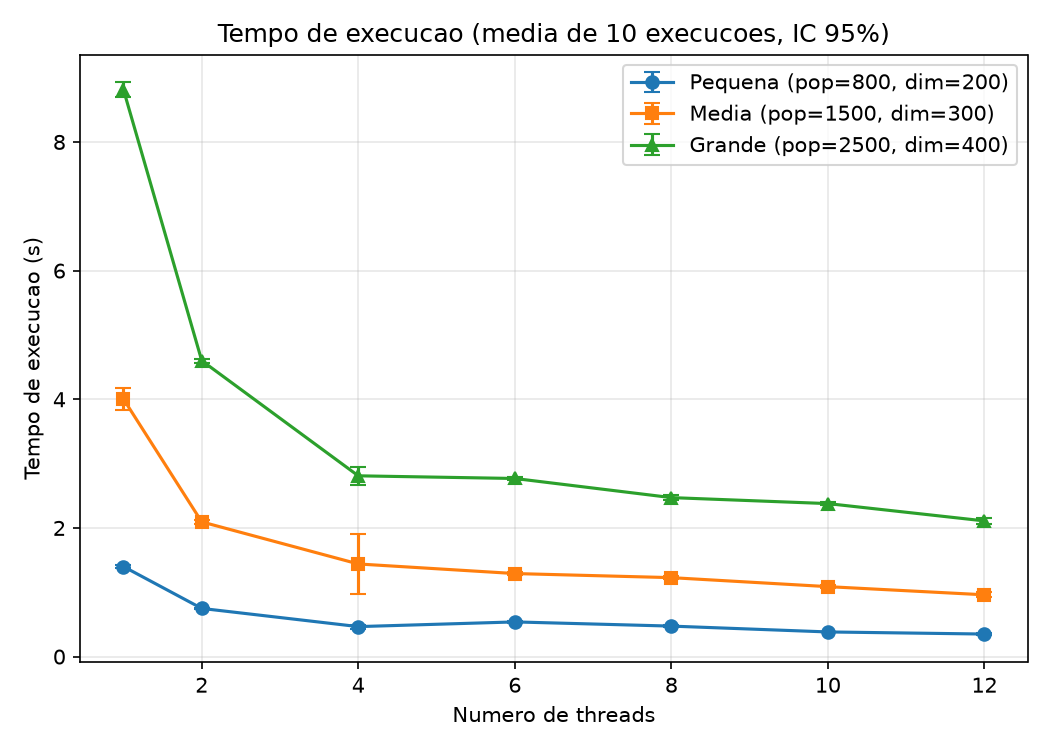
\includegraphics[width=.75\textwidth]{../results/tempo.png}
\caption{Tempo de execução (média de 10 execuções, IC 95\%) em função do
  número de threads, para os três tamanhos de entrada.}
\label{fig:tempo}
\end{figure}

A Figura~\ref{fig:speedup} mostra o speedup, comparado à reta de speedup ideal
(linear). A Figura~\ref{fig:eficiencia} apresenta a eficiência, e a
Figura~\ref{fig:karpflatt} a fração serial experimental estimada pela métrica
de Karp-Flatt.

\begin{figure}[ht]
\centering
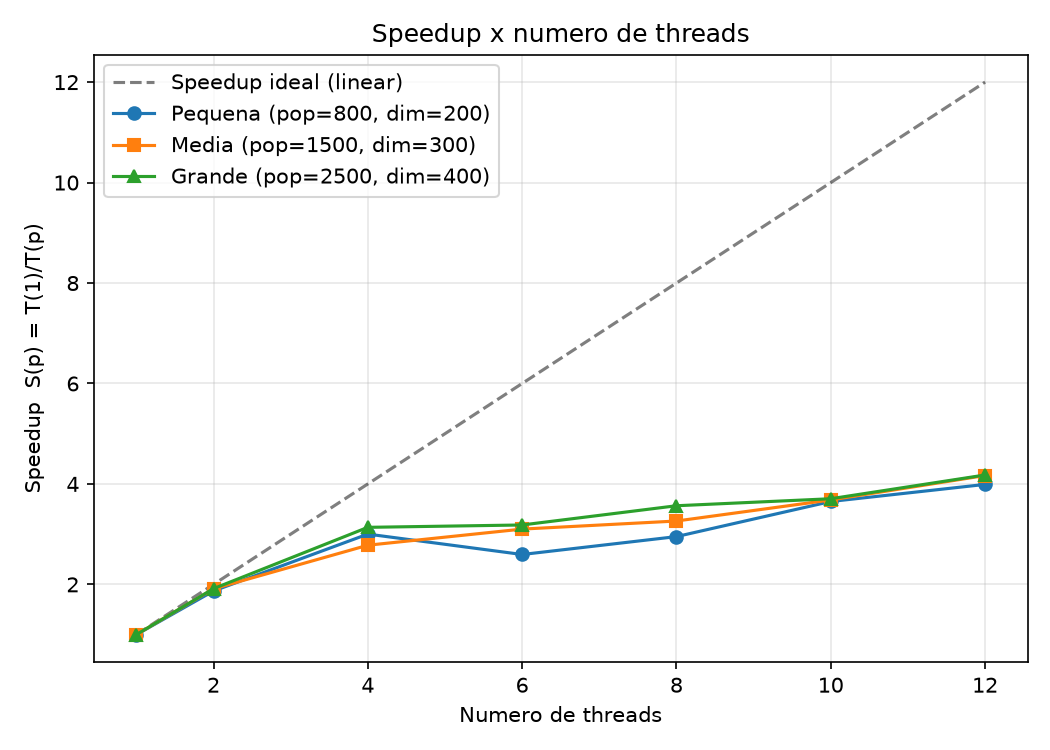
\includegraphics[width=.75\textwidth]{../results/speedup.png}
\caption{Speedup $S(p) = T(1)/T(p)$ em função do número de threads. A reta
  tracejada indica o speedup ideal (linear).}
\label{fig:speedup}
\end{figure}

\begin{figure}[ht]
\centering
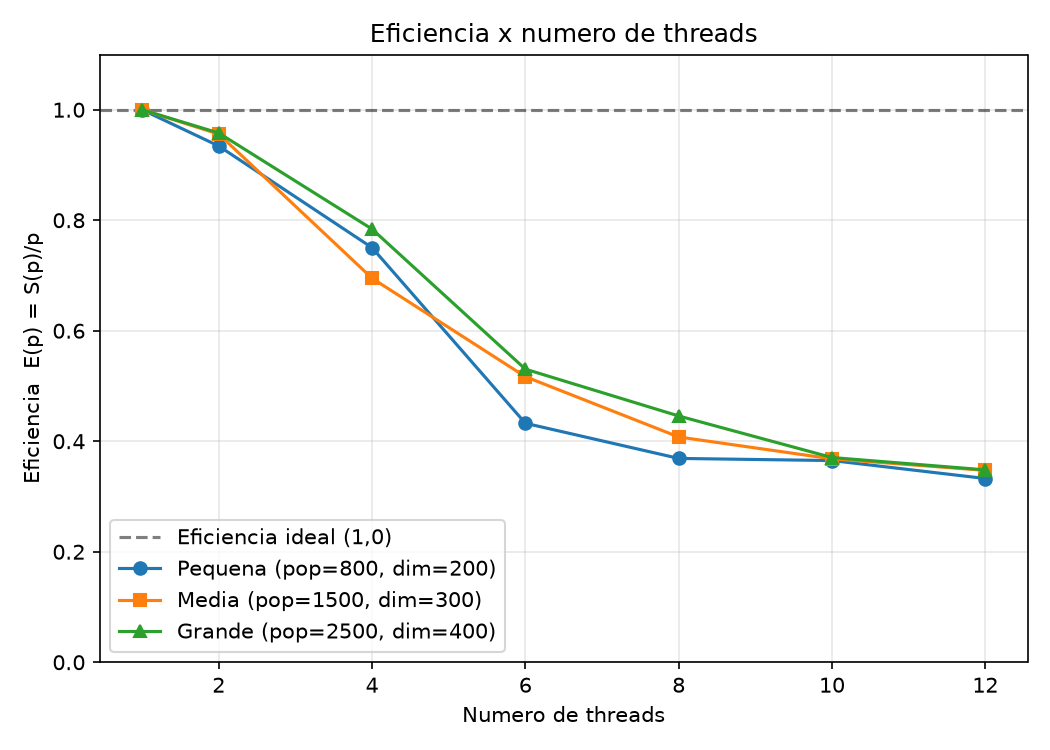
\includegraphics[width=.75\textwidth]{../results/eficiencia.png}
\caption{Eficiência $E(p) = S(p)/p$ em função do número de threads.}
\label{fig:eficiencia}
\end{figure}

\begin{figure}[ht]
\centering
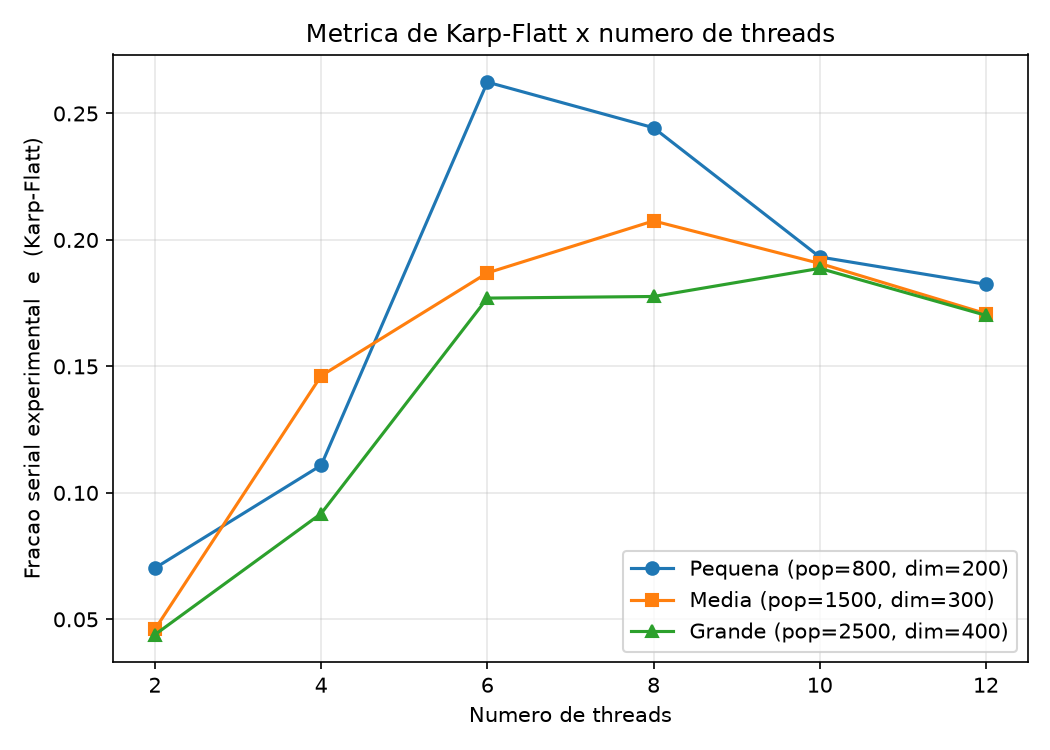
\includegraphics[width=.75\textwidth]{../results/karpflatt.png}
\caption{Métrica de Karp-Flatt (fração serial experimental) em função do
  número de threads.}
\label{fig:karpflatt}
\end{figure}

\section{Discussão}

Os resultados confirmam que a paralelização da avaliação de aptidão acelera
significativamente o AG. Para a entrada Grande, o tempo caiu de
$8{,}81$\,s (1 thread) para $2{,}11$\,s (12 threads), um speedup de
$4{,}18\times$. Contudo, esse ganho está muito abaixo do ideal linear de
$12\times$, e a eficiência despencou de $0{,}96$ (2 threads) para $0{,}35$
(12 threads). A seguir analisamos as causas.

\textbf{Efeito do tamanho da entrada.} Entradas maiores apresentam melhor
speedup e eficiência. Isso é coerente com a teoria: quanto maior a população e
a dimensão, maior o volume de trabalho \emph{paralelo} (avaliações de fitness)
em relação ao trabalho \emph{sequencial} fixo (seleção, crossover e mutação) e
ao overhead de criação/sincronização das threads. Ou seja, a fração serial
relativa diminui, aproximando-se do regime favorável da Lei de Amdahl.

\textbf{Arquitetura híbrida.} O ganho de desempenho não é uniforme ao longo do
eixo de threads. Até cerca de 4 threads, o trabalho é alocado nos
\emph{P-cores}, mais rápidos, e o speedup cresce de forma próxima à linear.
Entre 4 e 8 threads, passam a ser usados os \emph{E-cores}, mais lentos, de
modo que cada thread adicional contribui menos, e a eficiência cai. Acima de 8
threads, recorre-se ao \emph{Hyper-Threading} dos P-cores, em que duas threads
compartilham os recursos de um mesmo núcleo físico, resultando em ganho
marginal e, por vezes, em saturação do tempo. Esse comportamento explica a
inflexão observada nas curvas de speedup e eficiência.

\textbf{Karp-Flatt e overhead.} A métrica de Karp-Flatt torna esse diagnóstico
explícito. O crescimento da fração serial experimental $e$ com o número de
threads indica que a limitação não se deve apenas à fração serial intrínseca
do algoritmo (que seria constante), mas também ao \textbf{overhead paralelo
crescente} e à \textbf{heterogeneidade dos núcleos}. Em outras palavras, parte
da perda de eficiência observada não é culpa do algoritmo, e sim das
características físicas do processador e do custo de gerenciar muitas threads.

\textbf{Corretude.} Em todas as execuções, o melhor fitness obtido foi
idêntico independentemente do número de threads (para a mesma semente),
confirmando que a paralelização da avaliação de aptidão preserva exatamente a
semântica do AG sequencial, sem condições de corrida.

\section{Conclusões}

Este trabalho implementou um Algoritmo Genético em C++ para maximizar uma
função matemática de alto custo computacional (o negativo da função de
Rastrigin) e paralelizou sua etapa mais cara --- a avaliação de aptidão da
população --- utilizando OpenMP, no modelo mestre-escravo. A paralelização
exigiu uma alteração mínima do código (uma única diretiva
\texttt{\#pragma omp parallel for}) e preservou integralmente o resultado do
algoritmo.

Os experimentos, conduzidos com rigor estatístico (10 execuções, IC 95\%) em
um processador de arquitetura híbrida, mostraram speedups expressivos para
entradas grandes e evidenciaram, por meio das métricas de eficiência e de
Karp-Flatt, os limites da escalabilidade: a fração serial do algoritmo, o
overhead de gerenciamento das threads e, sobretudo, a heterogeneidade dos
núcleos (P-cores, E-cores e Hyper-Threading). Conclui-se que a paralelização
da avaliação de fitness é uma estratégia eficaz e de baixo custo de
implementação para acelerar Algoritmos Genéticos aplicados a funções caras,
desde que o volume de trabalho paralelo seja suficiente para amortizar o
overhead. Como trabalhos futuros, sugerem-se a fixação de afinidade de threads
aos P-cores, o uso de escalonamento dinâmico para balanceamento de carga entre
núcleos heterogêneos e a comparação com uma versão de memória distribuída
(MPI) ou em GPU.

\bibliographystyle{sbc}
\bibliography{sbc-template}

\end{document}
